%ustawienia
\documentclass[12pt,a4paper]{article}
\usepackage[T1]{fontenc}
\usepackage{mathptmx}
\usepackage[utf8]{inputenc}
\usepackage{amssymb}
\usepackage[polish]{babel}
\usepackage{polski}
\usepackage{amsmath}
\usepackage{amsfonts}
\usepackage[left=3.5cm,right=2cm,top=2.5cm,bottom=2.5cm]{geometry}
\usepackage{graphicx}
\usepackage{indentfirst} 
\usepackage{float}
\usepackage{hyperref}
\usepackage[most]{tcolorbox}
\usepackage{fancyhdr}
\setlength{\parindent}{0.7cm}
\hypersetup{
	colorlinks = true,
	linkcolor = black,
	filecolor = magenta,
	urlcolor = blue,
	}
\urlstyle{same}	
	
\author{
	\\\includegraphics[width=0.7\linewidth]{img/logoPWSZ.eps} \\\\\\\\
	\hfill Karpiński Maciej\\
	\hfill Krysa Marcin\\
	\hfill Kuczma Łukasz\\
	\hfill Mertuszka Adam\\\\
	\hfill Prowadzący mgr inż. Marcin Tracz
	}
\title{\textbf{Wprowadzenie do zarządzania projektami deweloperskimi}\\\line(1,0){400}\\\textbf{laboratorium}}
\date{}

\begin{document}

	%Stron tytułowa
	\maketitle
	\thispagestyle{fancy}
	\fancyhf{}
	\rhead{\textcolor{gray}{\footnotesize Państwowa Wyższa Szkoła Zawodowa im. Witelona w Legnicy\\Informatyka, rok III\\Semestr zimowy 2020/2021}}	
	\renewcommand{\headrulewidth}{0pt}
	\clearpage

	%Spis treści
	\pagestyle{fancy}
	\rfoot{\thepage}	
	\tableofcontents
	\newpage

	%opis projektu
	\section{Opis projektu}
		\indent Projekt ,,Magazynek piwosza'' jest aplikacją internetową przeznaczoną dla pasjonatów warzących piwo w domu, którzy chcieliby posiadać listę posiadanych składników.
		,,Magazynek piwosza'' pozwala zarejestrowanemu i zalogowanemu użytkownikowi na tworzenie swoich wirtualnych ,,schowków'' i przypisywania do nich
		składników wraz z ich datami ważności. Funkcjonalność aplikacji obejmuje:
		\begin{itemize}
			\item Dostęp do aplikacji poprzez przeglądarkę www (PC, smartphone)
			\item rejestrację i logowanie użytkowników,
			\item dodawanie, modyfikowanie i usuwanie kategorii przedmiotów,
			\item dodawanie, modyfikowanie i usuwanie przedmiotów,
			\item dodawanie, modyfikowanie i usuwanie magazynów,
			\item wysyłanie powiadomień o zbliżającym się terminie ważności,
		\end{itemize}		
	\newpage
	
	%Opis poszczególnych ról w grupie, kto za co był odpowiedzialny
	\section{Role w grupie}
	\indent Każdy z członków zespołu posiada następujące role:
	\begin{itemize}
		\item Karpiński Maciej:
			\begin{itemize}
				\item Backend
				\item Baza danych
				\item DevOps
				\item Dokumentacja
				\item Testy integracyjne
			\end{itemize}
		\item Krysa Marcin
			\begin{itemize}
				\item Frontend
			\end{itemize}
		\item Kuczma Łukasz
			\begin{itemize}
				\item Backend
			\end{itemize}
		\item Mertuszka Adam
			\begin{itemize}
				\item Frontend
				\item Lider
				\item Project Manager
			\end{itemize}
	\end{itemize}		
	\newpage
	
	%Opis wymagań i założeń projektowych
	\section{Wymagania i założenia projektowe}
		Wymagania projektowe:
		\begin{itemize}
			\item Uwierzytelnianie (w tym poprzez social media);
			\item Przechowywanie różnych typów produktów;
			\item Powiadomienia;
			\item Poręczny interfejs;
			\item Separacja backendu i frontendu;
			\item Logi.
		\end{itemize}
		Założenia:
		\begin{itemize}
			\item Użytkownik może tworzyć swoje własne schowki;
			\item Użytkownik wybiera składnik z listy składników i dodaje go do swojego schowka;
			\item Użytkownik wprowadza termin ważności składnika;
			\item Użytkownik dostaje powiadomienie o zbliżającym się terminie ważności;
			\item Przyjazny interfejs użytkownika;
		\end{itemize}				 
	\newpage
	
	%Opis działania aplikacji / systemu
	\section{Opis działania}
		\indent Aplikacja pierwotnie stworzona dla miłośników piwowarstwa, ma za zadanie pomóc w zarządzaniu składnikami w swoich magazynkach, które niezbędne
			są do warzenia piwa. Wszystkie dodane magazyny są indywidualne i spersonalizowane, stąd też program wymaga od użytkownika zalogowania się albo poprzez rejestrację
			na stronie, albo używając mediów społecznościowych (gmail, facebook). Aby użytkownik dodał swoje produkty, musi na samym początku dodać swój pierwszy magazyn.
			Składów może być wiele - użytkownik może je podzielić wedle uznania kategoriami lub użyć jednego magazynu, aby trzymać w nim wszystkie składniki.\\
		\indent Każdy produkt posiada swoją indywidualną datę przydatności do spożycia, dlatego też przy dodawaniu przedmiotu do magazynu, niezbędne jest podanie daty przydatności
			do spożycia.\\
		\indent Aplikacja raz dziennie zbiera wszystkie informacje na temat produktów dodanych w magazynach, sprawdza daty przydatności i wysyła spersonalizowane powiadomienia
			mailowe z informacją, który składnik przeterminuje się lub który już jest przeterminowany.\\
		\indent Gotowa aplikacja przystosowana będzie typowo pod miłośników piwowarstwa, więc użytkownicy, przy dodawaniu przedmiotów do swoich magazynów, będą mogli wybierać
			predefiniowane składniki tylko z kategorii ,,Piwowarstwa'', jednak aplikacja została stworzona w taki sposób, aby umożliwić przyszłościowo rozbudowanie
			bibliotek produktowych o np. ,,nabiał'', czy ,,produkty mięsne''.
	
	%Opis wykorzystanych technologii, narzędzi i rozwiązań technicznych
	\newpage
	\section{Wykorzystana technologia i narzędzia}
		\indent Przy tworzeniu projektu aplikacji wykorzystano następujące technologie:

		\subsection{ASP.NET Core 3.1}
			\indent ASP.Net Core jest wysokowydajnym frameworkiem, do budowania nowoczesnych aplikacji internetowych wykorzystujących moc obliczeniową chmur. ASP.Net Core jest technologią
			open - source, wykorzystującą silnik html Razor, dzięki której możliwe jest tworzenie aplikacji mulitplaformowych, które mogą być używane na każdym urządzeniu wyposażonym
			w przeglądarkę internetową.

		\subsection{AutoMapper}
			\indent AutoMapper jest biblioteką służącą do mapowania między obiektami, dzięki czemu można automatycznie mapować właściwości dwóch różnych obiektów,
					przekształcając obiekt wejściowy jednego typu na obiekt wyjściowy innego typu.  
		\subsection{C\#}
			\indent C\# jest obiektowym językiem programowania, zaprojektowanym w latach 1998 – 2001 dla firmy Microsoft.
			Napisany program jest kompilowany do Common Intermediate Language(CLI), który następnie wykonywany jest w środowisku uruchomieniowym takim jak .NET Framework,
			.NET Core, Mono lub DotGNU.
			Wykorzystanie CLI sprawia, że kod programu jest wieleplatformowy (dopóki istnieje odpowiednie środowisko uruchomieniowe).
			C\# posiada wiele wspólnych cech z językami Object Pascal, Delphi, C++ i Java a najważniejszymi cechami C\# są:
			\begin{itemize}
				\item Obiektowość z hierarchią o jednym elemencie nadrzędnym (podobnie jak w Javie);
				\item Zarządzaniem pamięcią zajmuje się środowisko uruchomieniowe;
				\item Właściwości i indeksery;
				\item Delegaty i zdarzenia – rozwinięcie wskaźników C++;
				\item Typy ogólne, generyczne, częściowe, Nullable, domniemane, anonimowe;
				\item Dynamiczne tworzenie kodu;
				\item Metody anonimowe;
				\item Wyrażenia lambda.
			\end{itemize}
		
		\subsection{Coverlet}
			\indent Coverlet to projekt typu open source, który zapewnia wieloplatformowy framework
			pokrywający kod. Coverlet zbiera dane dotyczące przebiegu testu pokrycia,
			które są używane do generowania raportów.
		
		\subsection{CSS}
			\indent Kaskadowe arkusze stylów (ang. Cascading Style Sheets, w skrócie CSS) – język służący do opisu formy prezentacji (wyświetlania) stron WWW.
				CSS został opracowany przez organizację W3C w 1996 r. jako potomek języka DSSSL przeznaczony do używania w połączeniu z SGML-em. Arkusz stylów CSS to lista
				dyrektyw (tzw. reguł) ustalających w jaki sposób ma zostać wyświetlana przez przeglądarkę internetową zawartość wybranego elementu (lub elementów)
				(X)HTML lub XML. Można w ten sposób opisać wszystkie pojęcia odpowiedzialne za prezentację elementów dokumentów internetowych, takie jak rodzina czcionek,
				kolor tekstu, marginesy, odstęp międzywierszowy lub nawet pozycja danego elementu względem innych elementów bądź okna przeglądarki.
				Wykorzystanie arkuszy stylów daje znacznie większe możliwości pozycjonowania elementów na stronie, niż oferuje sam (X)HTML. CSS został stworzony w celu
				odseparowania struktury dokumentu od formy jego prezentacji. Separacja ta zwiększa zakres dostępności witryny, zmniejsza zawiłość dokumentu, ułatwia wprowadzanie
				zmian w strukturze dokumentu. CSS ułatwia także zmiany w renderowaniu strony w zależności od obsługiwanego medium (ekran, palmtop, dokument w druku, czytnik ekranowy).
				Stosowanie zewnętrznych arkuszy CSS daje możliwość zmiany wyglądu wielu stron naraz bez ingerowania w sam kod (X)HTML, ponieważ arkusze mogą być wspólne dla wielu dokumentów. 		
		
		\subsection{Docker}
			\indent Docker jest otwarto źródłowym oprogramowaniem służącym do realizacji „konteneryzacji” aplikacji, służąca jako platforma dla programistów
				i administratorów do tworzenia, wdrażania i uruchamiania aplikacji rozproszonych. Pozwala umieścić program oraz jego zależności (biblioteki,
				pliki konfiguracyjne, lokalne bazy danych itp.) w lekkim, przenośnym, wirtualnym kontenerze, który można uruchomić na prawie każdym serwerze
				z systemem Linux. Kontenery wraz z zawartością działają niezależnie od siebie i nie wiedzą o swoim istnieniu. Mogą się jednak ze sobą
				komunikować w ramach ściśle zdefiniowanych kanałów wymiany informacji. Dzięki uruchamianiu na jednym wspólnym systemie operacyjnym,
				konteneryzacja jest lżejszym sposobem wirtualizacji niż pełna wirtualizacja lub parawirtualizacja za pomocą wirtualnych systemów
				operacyjnych.
				 	
		\subsection{Entity Framework}		 
		 	\indent Entity Framework jest technologią open - source do mapowania obiektowo – relacyjnego (ORM), które wspierają rozwój aplikacji zorientowanych na dane.
		 	Entity Framework umożliwia programistom pracę z danymi w postaci obiektów i właściwości specyficznych dla domeny, bez konieczności przejmowania się bazowymi
		 	tabelami i kolumnami baz danych, w których dane są przechowywane. 

		\subsection{Fluent Assertions}
			\indent Fluent Assertions to zestaw metod rozszerzających .NET, które pozwalają
			w bardziej naturalny sposób określić oczekiwany wynik testu jednostkowego.
			Umożliwia to prostą, intuicyjną budowę testu oraz szybsze diagnozowanie przyczyn
			niepowodzenia testu dzięki czytelniejszym błędom.
		\subsection{HTML}
			\indent HTML (ang. HyperText Markup Language) – hipertekstowy język znaczników, wykorzystywany do tworzenia dokumentów hipertekstowych. HTML pozwala opisać
				strukturę informacji zawartych wewnątrz strony internetowej, nadając odpowiednie znaczenie semantyczne poszczególnym fragmentom tekstu – formując hiperłącza,
				akapity, nagłówki, listy – oraz osadza w tekście dokumentu obiekty plikowe np. multimedia bądź elementy baz danych np. interaktywne formularze danych.
				HTML umożliwia określenie wyglądu dokumentu w przeglądarce internetowej. Do szczegółowego opisu formatowania akapitów, nagłówków, użytych czcionek i kolorów,
				zalecane jest wykorzystywanie kaskadowych arkuszy stylów.
				 
		\subsection{JavaScript}
			\indent JavaScript (w skrócie JS) – skryptowy język programowania, stworzony przez firmę Netscape Najczęściej spotykanym zastosowaniem języka JavaScript
				są strony internetowe. Skrypty te służą najczęściej do zapewnienia interakcji poprzez reagowanie na zdarzenia, walidacji danych wprowadzanych w formularzach
				lub tworzenia złożonych efektów wizualnych. Skrypty JavaScriptu uruchamiane przez strony internetowe mają znacznie ograniczony dostęp do komputera użytkownika.
				Po stronie serwera JavaScript może działać w postaci node.js lub Ringo. W języku JavaScript można także pisać pełnoprawne aplikacje. Fundacja Mozilla udostępnia
				środowisko złożone z technologii takich jak XUL, XBL, XPCOM oraz JSLib. Umożliwiają one tworzenie korzystających z zasobów systemowych aplikacji
				o graficznym interfejsie użytkownika dopasowującym się do danej platformy. Przykładem aplikacji napisanych z użyciem JS i XUL może być klient IRC o nazwie
				ChatZilla, domyślnie dołączony do pakietu Mozilla. Microsoft udostępnia biblioteki umożliwiające tworzenie aplikacji JScript jako część środowiska Windows
				Scripting Host. Ponadto JScript.NET jest jednym z podstawowych języków środowiska .NET. Istnieje także stworzone przez IBM środowisko SashXB dla systemu Linux,
				które umożliwia tworzenie w języku JavaScript aplikacji korzystających z GTK+, GNOME i OpenLDAP. Platforma Node.js umożliwia pisanie aplikacji wiersza poleceń oraz
				aplikacji serwerowych. Node.js używany jest także w środowisku Electron, który umożliwia pisanie aplikacji GUI. Język JavaScript używany jest także na urządzeniach
				internetu rzeczy, robotów czy układów takich jak Arduino poprzez bibliotekę Johnny-Five. 		
		
		\subsection{MailKit}
			\indent MailKit jest multiplatformową otwarto źródłową biblioteką .NET klienta pocztowego opartą o MimeKit, która została zoptymalizowana pod kątem urządzeń mobilnych.
			MailKit oferuje następującą funkcjonalność:
			\begin{itemize}
				\item Obsługa proxy HTTP, Socks4, Socks4a i Socks5;
				\item Uwierzytelnianie SASL;
				\item Kompletny klient SMTP;
				\item Kompletny klient POP3;
				\item Kompletny klient IMAP;
				\item Sortowanie i wątkowanie wiadomości po stronie klienta;
				\item Asynchroniczne wersje wszystkich metod sieciowych;
				\item Obsługa S/MIME, OpenPGP, DKIM i ARC;
				\item Obsługa Microsoft TNEF.
			\end{itemize}

		\subsection{Microsoft SQL Server}		 
		 	\indent Microsoft SQL Server jest systemem zarządzania relacyjnymi bazami danych opracowany przez firmę Microsoft. Cechą charakterystyczną jest głównie wykorzystywanie języka
		 	zapytań	Transact-SQL, który jest rozwinięciem standardu ANSI/ISO. W projekcie wykorzystano wersje 2019 Express, która jest bezpłatną edycją programu Microsoft SQL Server, oferująca
		 	podstawowy silnik bazy danych, nieposiadający ograniczenia ilości obsługiwanych baz lub użytkowników. Ograniczenia, występujące w wersji Express to  m.in.:
		 	korzystanie z~jednego procesora, 1 GB pamięci RAM, 10GB plików bazy danych czy brak SQL Agent.
		
		\subsection{Node.js}
		\indent Node.js – wieloplatformowe środowisko uruchomieniowe o otwartym kodzie do tworzenia aplikacji typu server-side napisanych w języku JavaScript.
			Przyczynił się do stworzenia paradygmatu ,,JavaScript everywhere'' umożliwiając programistom tworzenie aplikacji w~obrębie jednego języka programowania zamiast
			polegania na odrębnych po stronie serwerowej. Node.js składa się z silnika V8 (stworzonego przez Google), biblioteki libUV oraz kilku innych bibliotek.
			Domyślnym managerem pakietów dla Node.js jest Npm. 
		
		\subsection{Quartz.NET}
			\indent Quartz.NET jest otwarto źródłową biblioteką do planowania zadań.
				Quartz.NET może być używany do tworzenia prostych lub złożonych harmonogramów wykonywania
				dziesiątek, setek, a nawet dziesiątek tysięcy zadań.
				Quartz.NET jest portem biblioteki Quartz dla środowiska Java. 	 
		
		\subsection{React.js}
			\indent React.js – biblioteka języka programowania JavaScript, która wykorzystywana jest do tworzenia interfejsów graficznych aplikacji internetowych.
				Często wykorzystywana do tworzenia aplikacji typu Single Page Application. Z głównych cech wyróżniających bibliotekę React.js jest wirtualny DOM
				(Document Object Model). React przechowuje cały DOM aplikacji w pamięci, po zmianie stanu wyszukuje różnice między wirtualnym i prawdziwym DOM
				i aktualizuje zmiany. Drugą z cech szczególnych React jest język JSX. Jest on nakładką na JavaScript, która dodaje możliwość wstawiania kodu html
				(lub komponentów React) bezpośrednio w kodzie, zamiast ciągu znaków. React.js jest obecnie używany na stronach internetowych firm takich
				jak Netflix, Imgur, PayPal, Archive.org, Gamepedia, SeatGeek, HelloSign czy Walmart.

		\subsection{SEQ}
			\indent Seq jest zbudowany na potrzeby nowoczesnego, strukturalnego rejestrowania za pomocą szablonów wiadomości. Zamiast tracić czas i wysiłek na próbę
				wyodrębnienia danych z~dzienników w postaci zwykłego tekstu za pomocą delikatnego analizowania dziennika, właściwości skojarzone z każdym zdarzeniem
				dziennika są przechwytywane i wysyłane do Seq w czystym formacie JSON. Szablony wiadomości są obsługiwane natywnie przez ASP.NET Core, Serilog, NLog
				i wiele innych bibliotek. 

		\subsection{Serilog}
			\indent Serilog jest łatwą w konfiguracji biblioteką .NET zapewniającą podstawowe logowanie diagnostyczne do plików, konsoli itd. W przeciwieństwie do innych bibliotek
				rejestrowania dla .NET, parametry przekazywane wraz z komunikatami dziennika nie są destruktywnie renderowane do formatu tekstowego. Zamiast tego są zachowywane
				jako dane strukturalne, które można zapisać w formie dokumentu w magazynie danych NoSQL. Szablony komunikatów Serilog używają prostego DSL, który rozszerza
				zwykłe ciągi formatu .NET. Właściwości są nazywane w szablonie wiadomości i dopasowywane pozycyjnie z argumentami dostarczonymi do metody dziennika.
		
		\subsection{Swashbuckle}
			\indent Swashbuckle jest biblioteką, która dodaje zestaw narzędzi ,,Swagger" generujących automatycznie dokumentację API aplikacji,
				wyposażoną w przejrzysty interfejs użytkownika. Swashbuckle umożliwia również testowanie API. Dokumentacja jest dostępna pod adresem internetowym:
			\begin{tcolorbox}[minipage,colback=white,arc=0pt,outer arc=0pt, fontupper=\scriptsize]
				\center					
				\url{http://homebrew.tplinkdns.com:81/swagger}
			\end{tcolorbox}

		\subsection{xUnit.net}
			\indent xUnit.net to darmowe narzędzie typu open source służące do testowania jednostkowego
			przeznaczone dla platformy .NET Framework, napisane przez oryginalnego autora NUnit.
			xUnit.net współpracuje z platformami Xamarin, ReSharper, CodeRush i TestDriven.NET.
	
	\newpage

	%Opis event stormingu + zrzuty z modelowania (wyraźne)
	\section{Event storming}
		\indent Event Storming został przeprowadzony na portalu ,,Miro'' \url{https://miro.com/}, w dniu 13.12.2020 było to nowe i ciekawe doświadczenie dla każdego z członków zespołu.
		Projekt w momencie przeprowadzenia event stormingu był już w zaawansowanej formie, wraz z rozpisanymi zadaniami więc wykorzystaliśmy spotkanie
		do stworzenia modelu pracy aplikacji.\\
		\indent Podczas tworzenia wizualizacji okazało się, że rozumienie aspektów działania i reagowania aplikacji na niektóre zdarzenia
		różnią się między poszczególnymi członkami zespołu, ujawnione różnice w wyobrażeniu na temat funkcjonowania poszczególnych komponentów aplikacji spowodowały dyskusje
		nad wyborem najlepszego rozwiązania. Podczas spotkania wyraźnie było widać brak doświadczenia w tego typu zadaniu, na początku często przerywaliśmy sobie wypowiedzi ale dość szybko
		doszliśmy do porozumienia i zapanował porządek. W miarę rozwoju aplikacji do modelu były dodawane kolejne szczegóły. 
		Wynikiem event stormingu jest spójny model działania aplikacji, dzięki czemu każdy członek zespołu może prześledzić przepływ informacji.
		\begin{figure}[H]
			\centering
			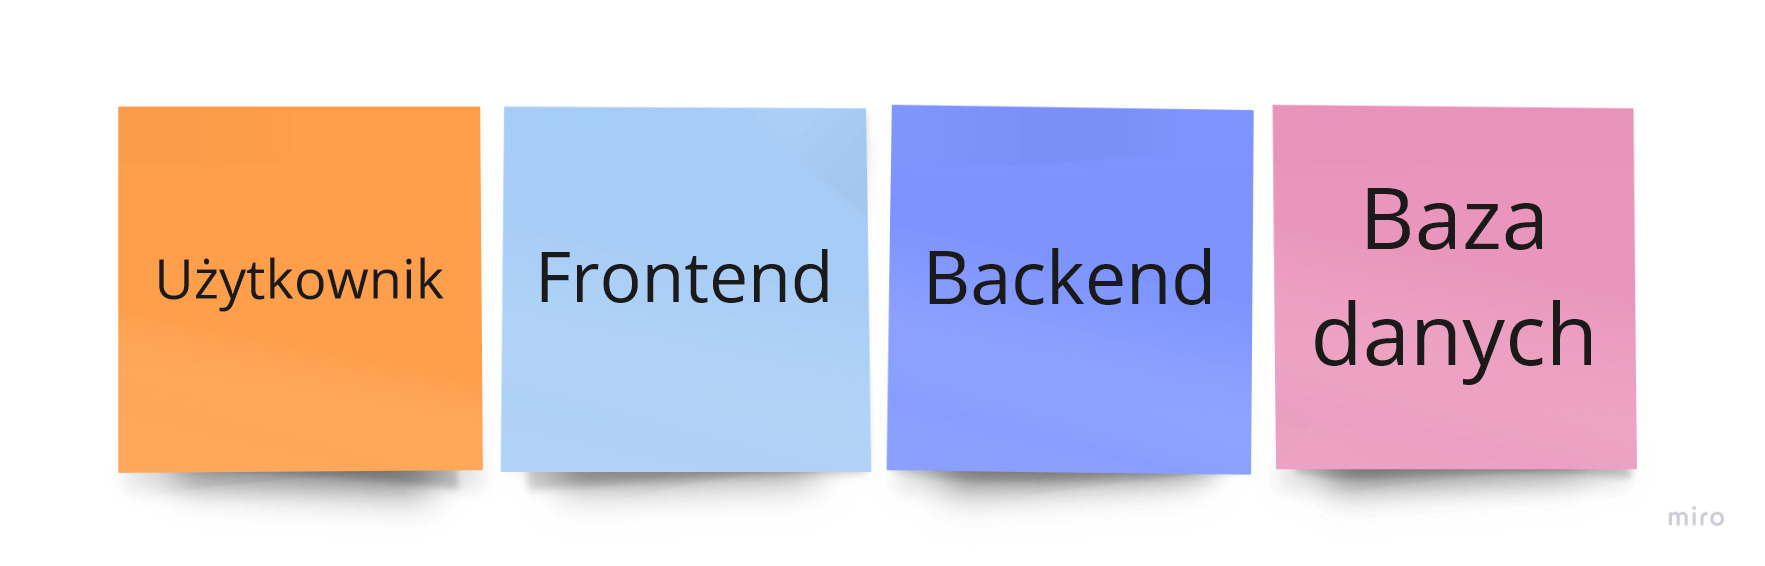
\includegraphics[width=0.6\textwidth]{img/miro_2.jpg}
			\caption{Miro - Legenda}
			\label{fig:miro-legenda}
		\end{figure}				
		\begin{figure}[H]
			\centering
			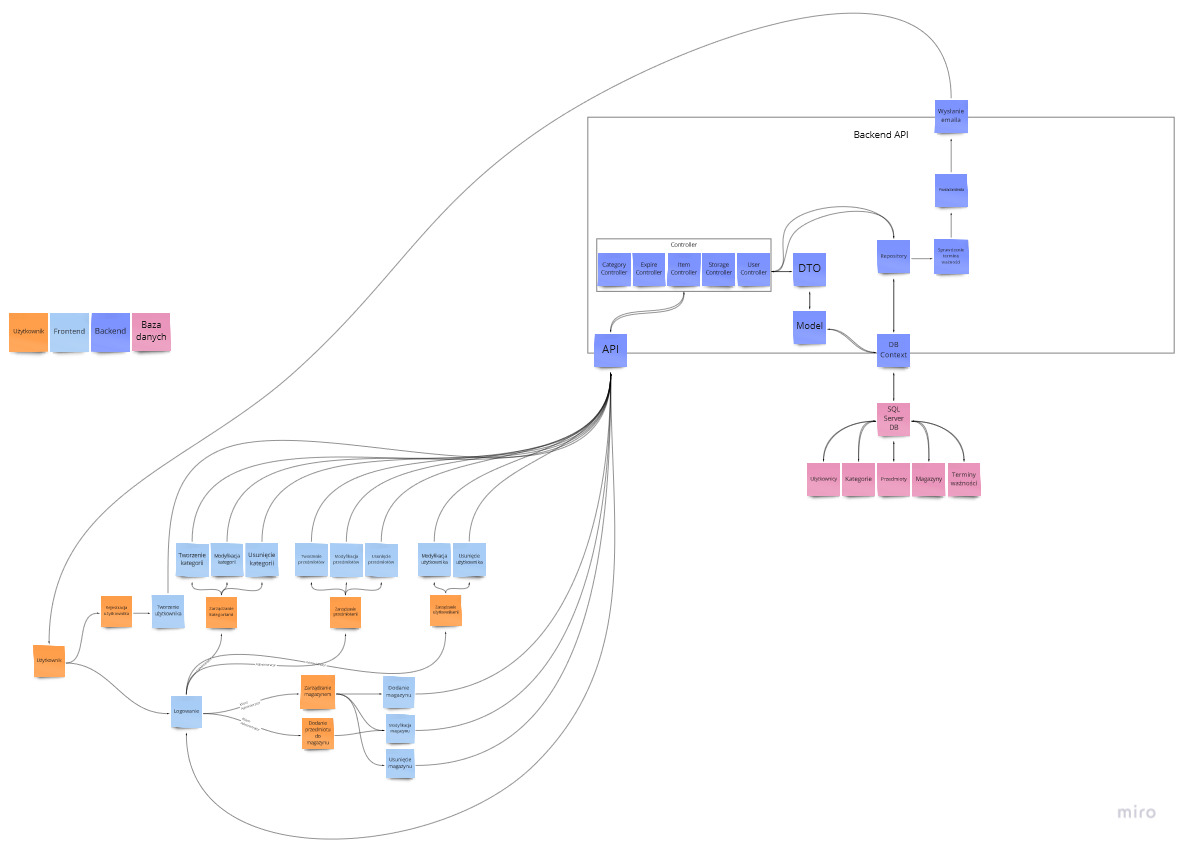
\includegraphics[width=\textwidth]{img/miro_1.jpg}
			\caption{Miro - Schemat działania aplikacji}
			\label{fig:miro-ogolne}
		\end{figure}
		\begin{figure}[H]
			\centering
			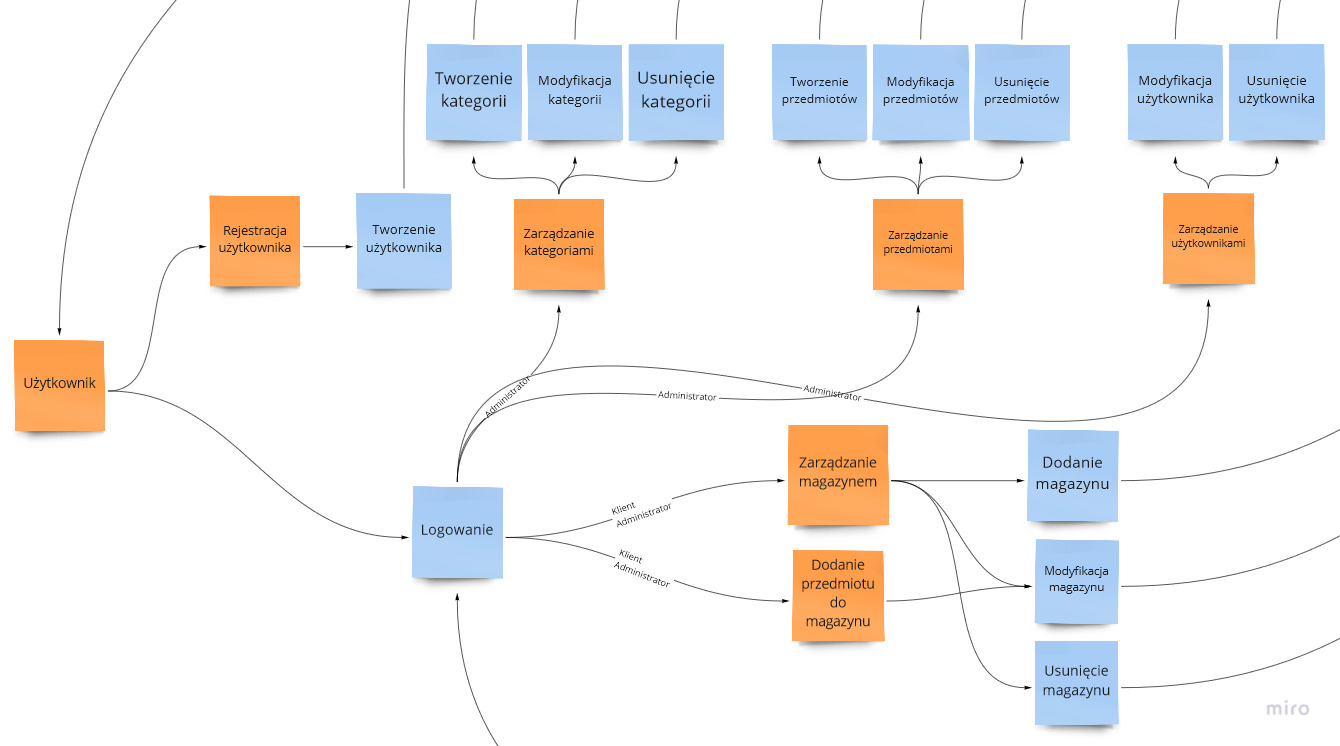
\includegraphics[width=\textwidth]{img/miro_4.jpg}
			\caption{Miro - Frontend aplikacji}
			\label{fig:miro-front}
		\end{figure}
		\begin{figure}[H]
			\centering
			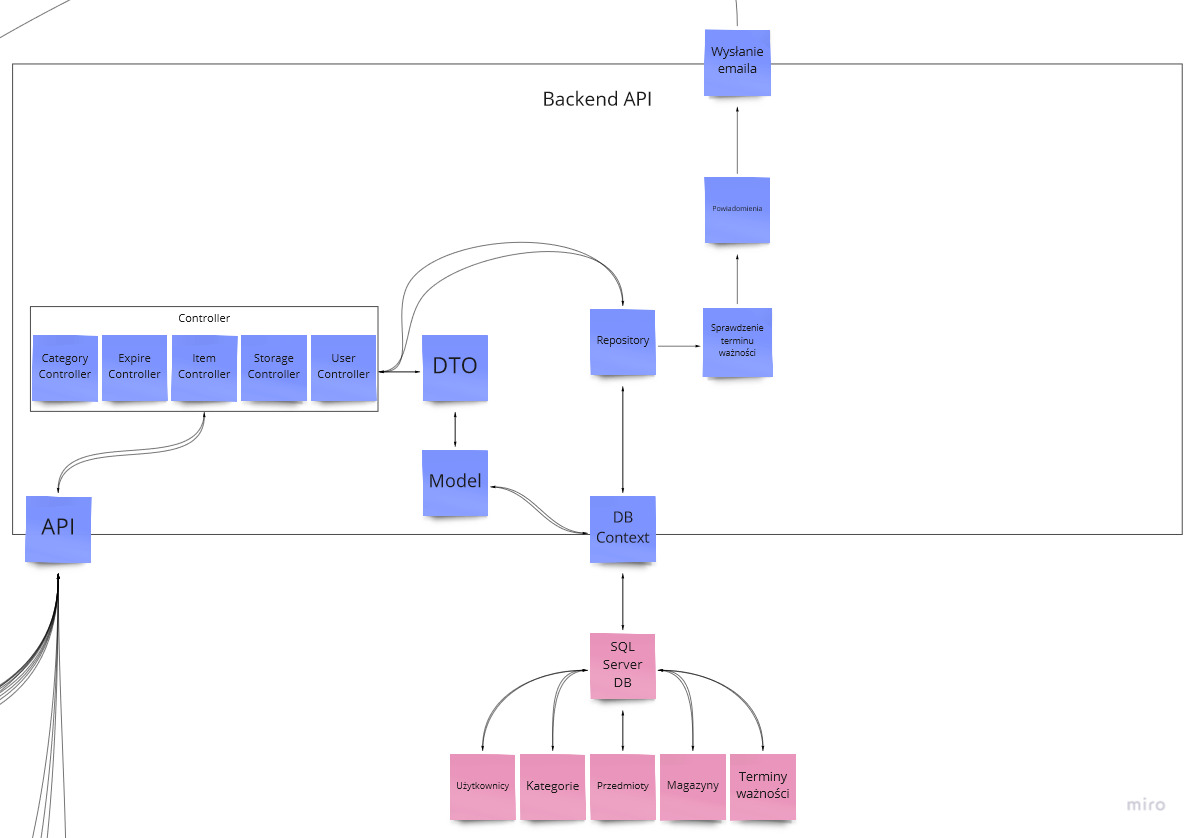
\includegraphics[width=\textwidth]{img/miro_3.jpg}
			\caption{Miro - Backend aplikacji}
			\label{fig:miro-backend}
		\end{figure}
	\newpage
	
	%Backlog
	\section{Backlog}
		\indent Backlog zaplanowanych działań został rozpisany na platformie ,,Trello''\\
		\begin{figure}[H]
			\centering
			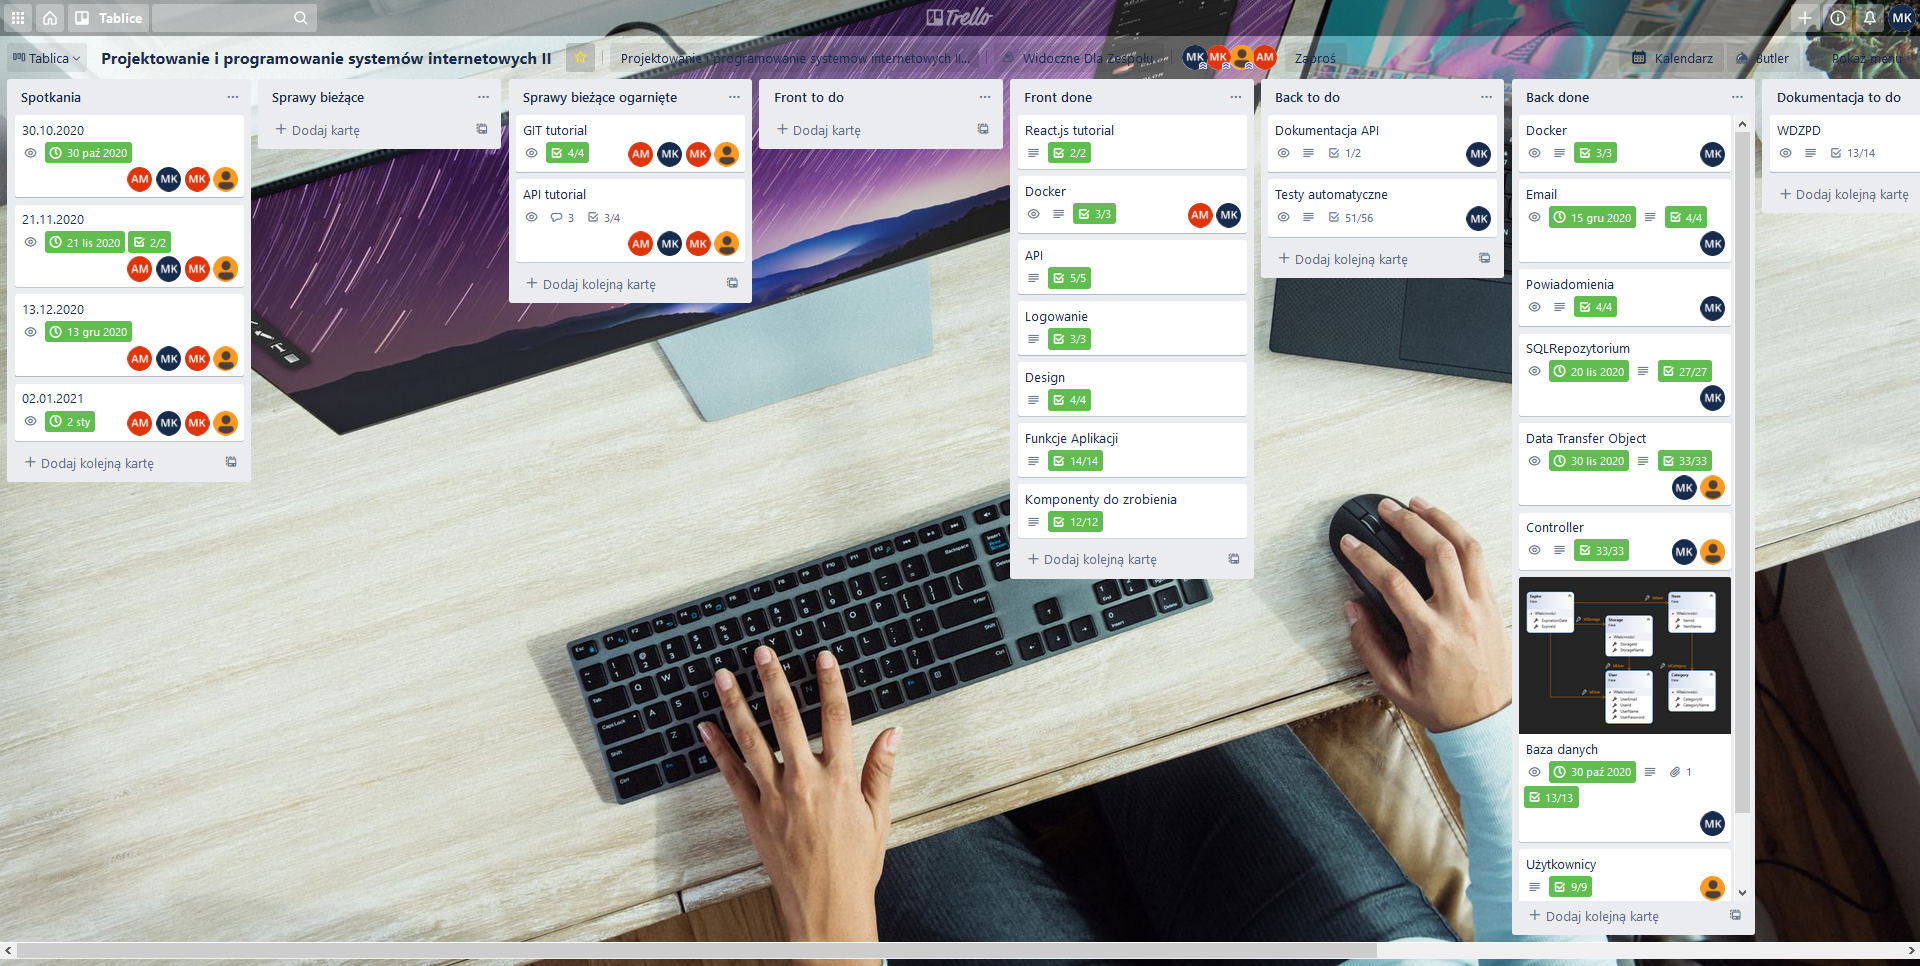
\includegraphics[width=\textwidth]{img/backlog.png}
			\caption{Backlog na platformie Trello}
			\label{fig:trello-backlog}
		\end{figure}
		\begin{figure}[H]
			\centering
			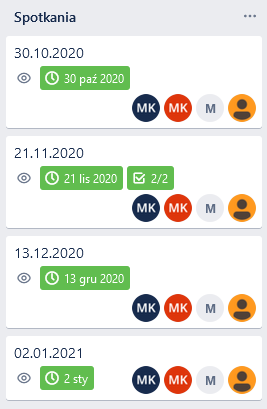
\includegraphics[width=0.5\textwidth]{img/spotkania.png}
			\caption{Terminy spotkań}
			\label{fig:trello-spotkania}
		\end{figure}
		\begin{figure}[H]
			\centering
			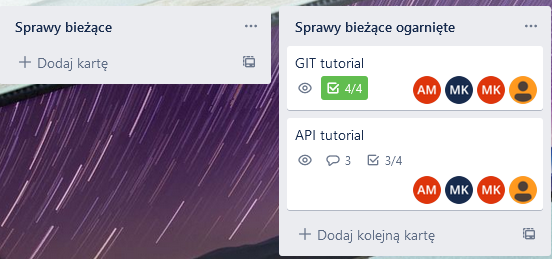
\includegraphics[width=\textwidth]{img/sprawy_biezace.png}
			\caption{Sprawy bieżące}
			\label{fig:trello-sprawy}
		\end{figure}
		\begin{figure}[H]
			\centering
			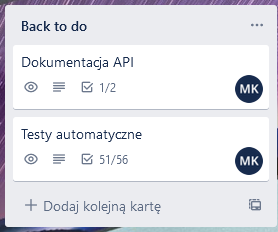
\includegraphics[width=0.5\textwidth]{img/backend_niedokonczony.png}
			\caption{Backend - TODO}
			\label{fig:trello-backend-to-do}
		\end{figure}
			\begin{figure}[H]
			\centering
			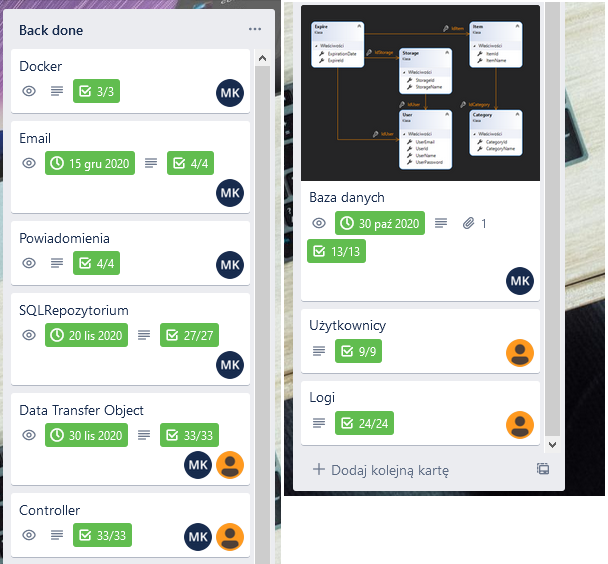
\includegraphics[width=\textwidth]{img/backend_done.png}
			\caption{Backend - Zrealizowane}
			\label{fig:trello-backend-done}
		\end{figure}
		\begin{figure}[H]
			\centering
			
\includegraphics[width=\textwidth]{img/dokumentacja.png}
			\caption{Dokumentacja}
			\label{fig:trello-doc}
		\end{figure}
		\begin{figure}[H]
			\centering
			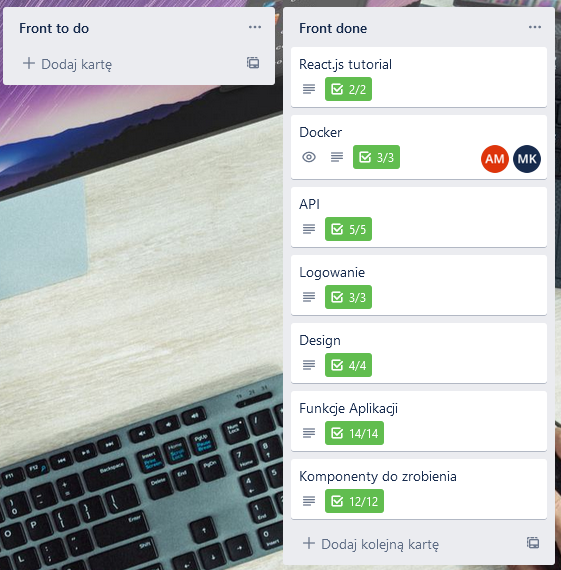
\includegraphics[width=\textwidth]{img/frontend.png}
			\caption{Frontend}
			\label{fig:trello-front}
		\end{figure}
	\newpage
	
	%Estymata
	\section{Estymata}
		\indent Szacowana estymacja poszczególnych części realizacji projektu:
		\begin{itemize}
			\item Backend:
				\begin{itemize}
					\item Autoryzacja: 10 godzin,
					\item Data Transfer Object (DTO): 2 godziny,
					\item DevOps: 5 godzin,
					\item End Point: 15 godzin,
					\item Harmonogram: 3 godziny,
					\item Logi: 10 godzin,
					\item Programowanie logiki aplikacji: 50 godzin,
					\item SQL Repozytorium: 3 godziny,
					\item Testy integracyjne: 10 godzin,
					\item Uwierzytelnianie: 10 godzin, 
					\item Wysyłanie e-maili: 30 minut,
				\end{itemize}
			\item Baza danych:
				\begin{itemize}
					\item Konfiguracja: 30 minut,
					\item Projekt tabel: 2 godziny,
				\end{itemize}
			\item Dokumentacja projektu: 5 godzin,
			\item Frontend: 
				\begin{itemize}
					\item Api: 10 godzin,
					\item Logowanie: 2 godziny,
					\item DevOps: 3 godziny,
					\item Design Aplikacji: 5 godzin,
					\item Konstruowanie aplikacji: 8 godzin,
					\item Tworzenie komponentów: 10 godzin,
					\item Pisanie funkcji: 15 godzin,
				\end{itemize}
			\item Zarządzanie projektem:
				\begin{itemize}
					\item Rozpisanie backlogu: 2 godziny,
					\item Rozpisanie sprintów: 2 godziny,
				\end{itemize}
		\end{itemize}				

	\newpage

	%Opis sprintów + zrzuty
	\section{Sprinty}
		\indent Ze względu na różne harmonogramy pracy zawodowej poszczególnych członków zespołu, trudno było wyznaczyć szczegółowy termin realizacji pojedynczych komponentów aplikacji,
		więc zostały wyznaczone jedynie ostateczne terminy elementów, na których bazują inne części aplikacji. Pozostałe elementy były realizowane w drugiej kolejności.\\
		\indent Backend:
		\begin{figure}[H]
			\centering
			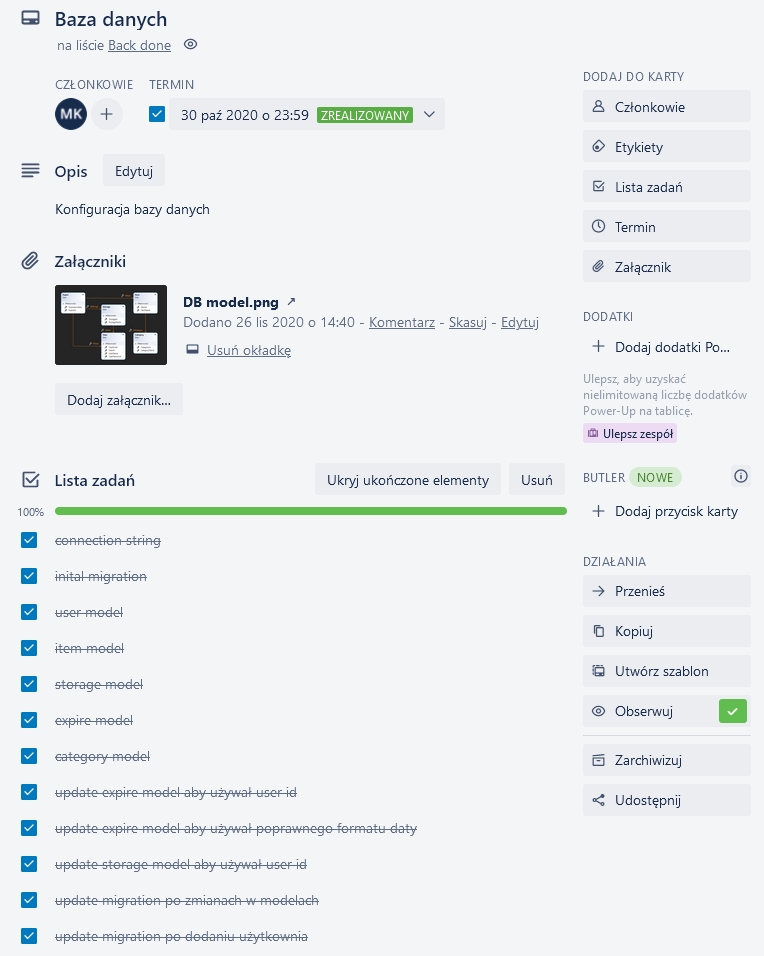
\includegraphics[width=\textwidth]{img/DBSprint.png}
			\caption{Sprinty - Baza danych}
			\label{fig:sprint-db}
		\end{figure}
				\begin{figure}[H]
			\centering
			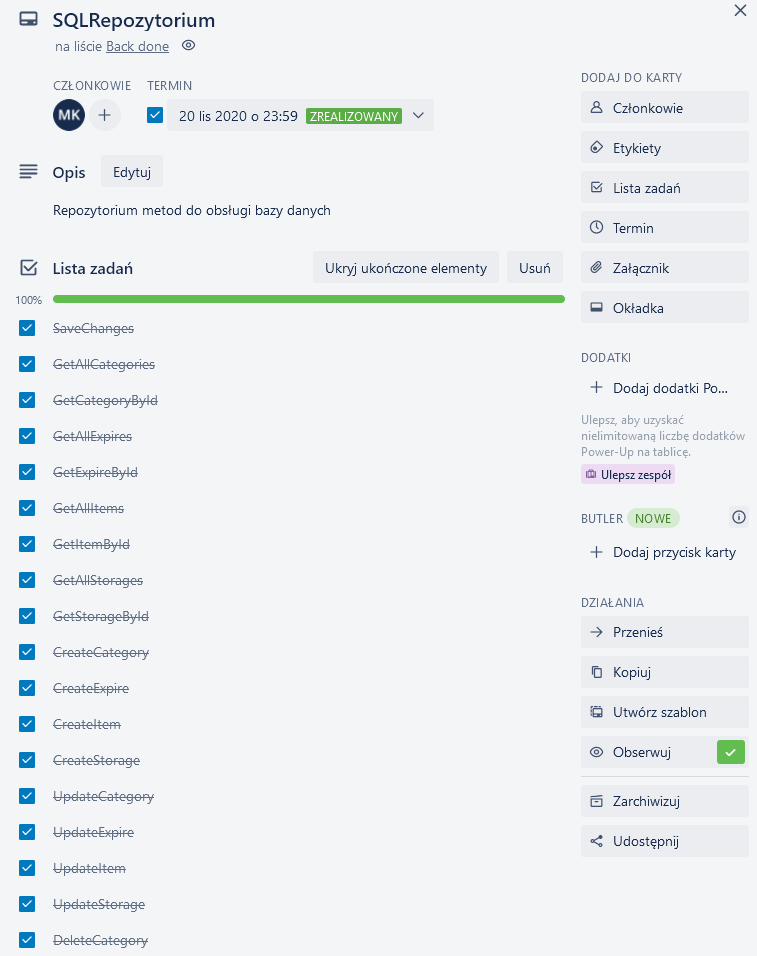
\includegraphics[width=\textwidth]{img/SQLRepo_Sprint.png}
			\caption{Sprinty - Repozytorium SQL}
			\label{fig:sprint-SQLRepo}
		\end{figure}
				\begin{figure}[H]
			\centering
			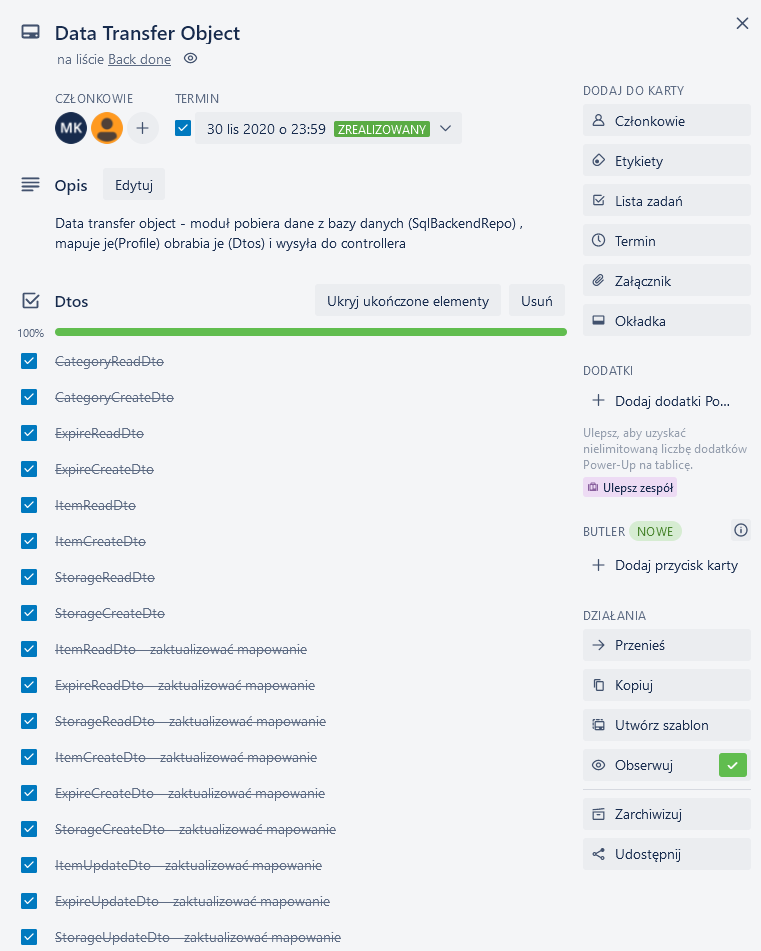
\includegraphics[width=\textwidth]{img/DTO_Sprint.png}
			\caption{Sprinty - Data Transfer Object}
			\label{fig:sprint-dto}
		\end{figure}
				\begin{figure}[H]
			\centering
			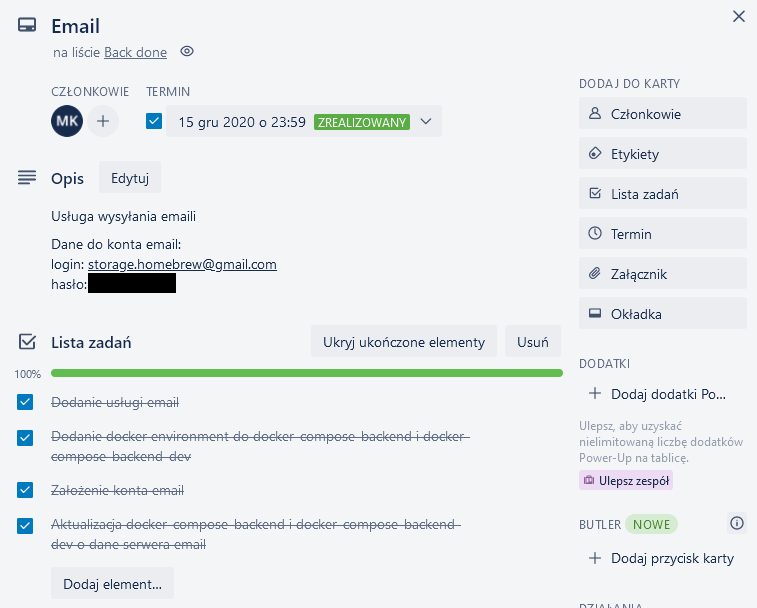
\includegraphics[width=\textwidth]{img/Email_sprint.png}
			\caption{Sprinty - usługa wysyłania e-maili}
			\label{fig:sprint-email}
		\end{figure}
	\newpage
	
	%Interfejs aplikacji (zrzuty) + krótki opis
	\section{Interfejs aplikacji}
	\newpage
	
	%Informacje uruchomieniowe w środowisku developerskim (instrukcja, co zrobić aby po ściągnięciu projektu z repozytorium GIT, móc uruchomić go na lokalnej maszynie)
	\section{Uruchomienie w środowisku developerskim}
		\indent Repozytorium kodu projektu i jego dokumentacja znajdują się w serwisie ,,GitHub'' pod adresem: 
			\begin{tcolorbox}[minipage,colback=white,arc=0pt,outer arc=0pt, fontupper=\scriptsize]
				\center
				\url{https://github.com/MacKarp/Homebrewing-storage}
			\end{tcolorbox}
		\indent Do uruchomienia systemu wymagana jest działająca platforma konteneryzacji ,,Docker''
			oraz narzędzie ,,Docker Compose'' szczegóły instalacji i konfiguracji wymaganych
			komponentów, można sprawdzić na stronie internetowej: \url{https://docs.docker.com/}.\\
		\indent Po ściągnięciu repozytorium w katalogu głównym projektu znajdują się pliki wsadowe, umożliwiające kompilację i uruchomienie ,,frontendu'' i ,,backendu''
		wraz z bazą danych.
		Pliki wsadowe dla systemu Windows:
		\begin{itemize}
			\item Backend-Start.bat
			\item Backend-Start-DEV.bat
			\item Backend-Stop.bat
			\item Backend-Stop-DEV.bat
			\item Frontend-Start.bat
			\item Frontend-Start-DEV.bat
			\item Frontend-Stop.bat
			\item Frontend-Stop-DEV.bat
		\end{itemize}
		Pliki dla systemu Linux:
		\begin{itemize}
			\item Backend-Start.sh
			\item Backend-Start-DEV.sh
			\item Backend-Stop.sh
			\item Backend-Stop-DEV.sh
			\item Frontend-Start.sh
			\item Frontend-Start-DEV.sh
			\item Frontend-Stop.sh
			\item Frontend-Stop-DEV.sh
		\end{itemize}
		\indent Pliki ,,Backend-Start.bat'', ,,Backend-Stop.bat'' oraz ,,Backend-Start.sh'' i ,,Backend-Stop.sh'' służą do uruchomiania i zatrzymywania ,,backendu'' w wersji produkcyjnej,
			która pobierze i~uruchomi najnowszą stabilną wersję ,,backendu'' aplikacji i bazę danych z serwisu ,,Docker Hub'', w przypadku pliku z przyrostkiem ,,DEV''
			zostanie uruchomiona kompilacja wersji deweloperskiej znajdującej się w lokalnym katalogu ,,Backend'' a następnie zostanie utworzony kontener z działającą aplikacją.
			W przypadku chęci zmiany ustawień ,,backendu'' aplikacji lub kontenera należy edytować - zachowując odpowiednie formatowanie plików yaml - plik w wersji produkcyjnej
			lub deweloperskiej:
		\begin{itemize}
			\item docker-compose-backend.yaml
			\item docker-compose-backend-dev.yaml		
		\end{itemize}
			\indent Pliki ,,Frontend-Start.bat'', ,,Frontend-Stop.bat'' oraz ,,Frontend-Start.sh'' i ,,Frontend-Stop.sh'' służą do uruchomiania i zatrzymywania ,,frontendu''
			aplikacji w wersji produkcyjnej,
			która pobierze i~uruchomi najnowszą stabilną wersję ,,frontendu'' z serwisu ,,Docker Hub'', w przypadku pliku z przyrostkiem ,,DEV''
			zostanie uruchomiona kompilacja wersji deweloperskiej znajdującej się w lokalnym katalogu ,Frontend'' a następnie zostanie utworzony kontener z działającą aplikacją.
			W przypadku chęci zmiany ustawień ,,frontendu'' aplikacji lub kontenera należy edytować - zachowując odpowiednie formatowanie plików yaml - plik w wersji produkcyjnej
			lub deweloperskiej:
		\begin{itemize}
			\item docker-compose-frontend.yaml
			\item docker-compose-frontend-dev.yaml		
		\end{itemize}
		\indent Domyślna konfiguracja znajdująca się w repozytorium umożliwia osobne uruchomienie ,,frontendu'' i ,,backendu'' wraz z bazą danych na jednym komputerze.
			Poszczególne komponenty aplikacji są dostępne pod adresami:
		\begin{itemize}
			\item Backend: \url{http://localhost:8080}
			\item Frontend: \url{http://localhost:3000}
			\item Logi: \url{http://localhost:5341}
		\end{itemize}
		\indent Domyślne dane dostępowe do bazy danych:
		\begin{itemize}
			\item Nazwa użytkownika: SA
			\item Hasło użytkownika: ThisIsNotSuperSecretP@55w0rd
			\item Adres: localhost
			\item Port: 14331
		\end{itemize}
			
	\newpage	
	
	%Podsumowanie, wnioski
	\section{Podsumowanie}
		\indent Sprawne zarządzanie projektem jest trudnym zadaniem i wymaga aby lider projektu był osobą charyzmatyczną.\\
		\indent Zarządzanie zespołem, w którym każdy z członków
		posiada różny harmonogram pracy zawodowej sprawiło wiele problemów organizacyjnych, często każdy z członków zespołu był dostępny w innym terminie,
		przez co ustalenie terminu spotkania online, w którym każdy z członków zespołu byłby dostępny było trudnym zadaniem, z tego powodu w czasie trwania projektu dominowała
		komunikacja pisana. Z tych samych względów rozpisywanie sprintów ograniczyło się jedynie do określenia nieprzekraczalnego terminu ukończenia elementów, od których inne
		komponenty projektowanej aplikacji były uzależnione, pozostałe elementy nie posiadały ściśle określonego terminu i były realizowane w drugiej kolejności.\\
		\indent Każdy z członków zespołu zdobył dużo wiedzy na temat pracy w zorganizowanym zespole, a także poznał narzędzia ułatwiające pracę w takim zespole.\\
		\indent Wspólnie doszliśmy do wniosku że Event Storming był nowym i  ciekawym doświadczeniem, chodź lepszym byłoby spotkanie ,,twarzą w twarz''
		wraz z osobą doświadczoną, która mogłaby poprowadzić takie spotkanie.\\
		\indent Wszyscy członkowie zespołu zgodnie stwierdzili że największym problem podczas pracy był problem z bieżącą komunikacją oraz z początkowym brakiem zrozumienia działania
		tablic na platformie ,,Trello'', raz zdarzyło się nawet	że dwie osoby zrobiły tą samą część aplikacji - na szczęście strata czasu w tym wypadku była mała.
	
	\newpage	
	\section{Spis rysunków}
		\listoffigures
\end{document}